\chapter{Experimental and Investigative Methods}

\section{Development Process}

During the initial survey we have seen many approaches for aircraft stability and
movement detection of \UAV. The most of these approaches were developed
iterative under consideration of the upcoming problems and obstacles 
\citebib[Iterative Development, Single and Dual Camera Feedback]
{AltOstMah02, AltOstTay03}
\citebib[Iterative Development, Landing and Position Control Development]
{LanSuePro08, LanSuePro09}. This procedure model also will be appropriate to this project, because the potential risks are difficult to identify. So the outcome of the development process have to be a
prototype which can be evaluated, tested and extended. A process model, which
provides an appropriate structure to face the iterative prototyping strategy
under the consideration of the risk aspects, is given with the spiral model. The
classical spiral model has typically four phases in which the product is
developed in an incremental evolutionary process. Derivates of this classical
model which focus the customer evaluation for quality improvements may three,
five or six phases. In the context of this project, the classical four phases
spiral model is used for scientific and feasibility study and does not have to
provide further customer communication phases
\citebib[pp.36-38 The Spiral Model]{Pre01}.

\newpage
A typical cycle of the four phases spiral model (\ref{fig:SpiralModelAndMBD})
 begins with the identification of
the objectives which have to be elaborated like performance,
functionality, flexibility and so far. The next step is to evaluate the
alternatives relative to the objectives and constraints and to determine
significant sources of risks. After that, the next level
iteration of the product is planned. In the special case of this project it is
comfortable to use \MBD in this phase by using the results of the previous phase as input.
This input can be a planed prototype or requirements which describe the changes
to execute. The output of the \MBD phase can be used again in the planning phase
for the next iteration \citebib
[pp.64-69 Spiral Model of the Software Process]{Boe88}.


\begin{figure}[!htbp]
	\centering
		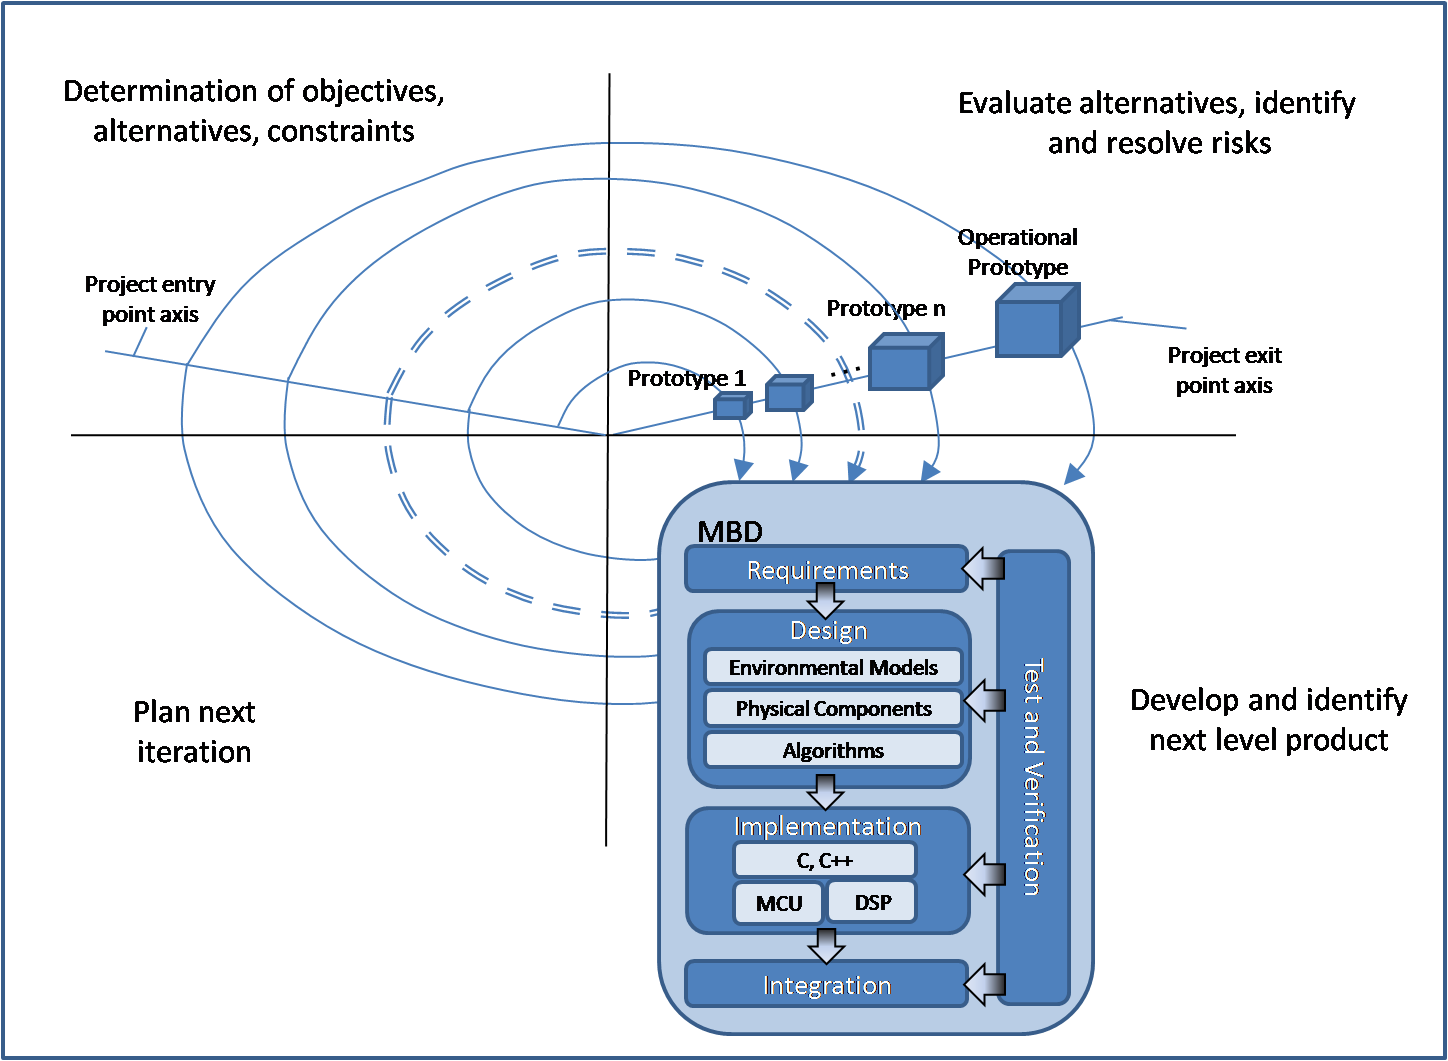
\includegraphics[width=0.75\textwidth]{graphic/SpiralModelAndMBD.png}
\caption
{The Spiral Model in combination with Model Based Design}
	\label{fig:SpiralModelAndMBD}
\end{figure}

\newpage
\section{Model Based Design}

\MBD is a popular method to encounter problems which come up in the development
of mechatronic products. These systems almost involve mechanical, electrical, control
 and embedded components which are developed in different teams of
engineers with a specialized focus on the part of the complete project. Some of
these components are related on the results of other components before they can
be developed. This problem can be solved with Model Based Design and the
advantage to develop modules of the complete project by simulating their
environment. So the development can run highly parallel with the benefit that the
modules can be continuous tested in each phase of the project
\citebib[pp.1-2 Challenges of mechatronic product development]{EasLamTur09}.

The development section in figure \ref{fig:SpiralModelAndMBD} includes the phases
and the corresponding key capabilities of \MBD. The first phase of \MBD is the
realization of the researched and required components into a simulation
environment. Thereby physical components, environmental model and algorithms are
abstracted to systems by using domain-specific modeling tools with a well
defined edges and intercommunication. The developed systems in the design phase
can be tested simultaneously to analyze the system performance and correctness.
Other key capabilities of \MBD are given in the implementation phase. The \MBD
tool Matlab allows to generate embedded code from the designed systems or to
combine handwritten code with the build simulation of the design phase. So the
implemented modules can be similarly tested in the adopted simulation
environment. Finally components which have passed the tests at the implementation
phase can be integrated together.\newpage Ultimately the final product can also be tested
with the \MBD tool by simulating the environment of the product e.g. in a \HIL
test bench. \citebib[Model Based Design, MathWorks]{Mat10}

\section{Overall Design Model}
The overall design model gives an overview of the components of the simulation
which has to be realized in the context of this project and the corresponding
applied techniques. As visualised in figure \ref{fig:InitialDesign}, the left
side of the simulation abstracts the embedded system of the quadrocopter. Inside
these components the plant or physical model has to simulate the movement
behaviour in the \DOF of the quadrocopter. Furthermore the controller has to
correct the position of the \UAV and to compensate outside disturbances with
information of the \IMU and the distributed correction value of the base station.
The environment simulation which has to include the underground and disturbances
simulation will be triggered to start just as the rest of the simulation with a
task which describes the ideal flight manoeuvre. The transmissions of the camera
\IMU and correction data have to be delayed in relation to a configurable
transmission rate. The image processing has to be executed with an application,
realized in OpenCV \citebib[OpenCV Project]{OpenCV2_0} and invoked by Matlab
\citebib[OpenCV and MEX-Functions in Matlab]{EsmSna08}. The calculated drift from
image processing finally has to be compared with the received values of the \IMU
to determine the position correction value. This correction has to be
transmitted to the embedded system and included in the correction of the controller.
\newpage
 The novel aspect of the project here is reflected in the approach to simulate
 the complete embedded system, the transmission process, the base station and to realize the
image processing in an application. The strength of this approach is that the
simulation gives better results and a deep insight to the concurrent processes
and helps to understand the challenges and limitations of the investigated
scheme.


\begin{figure}[!htbp]
	\centering
		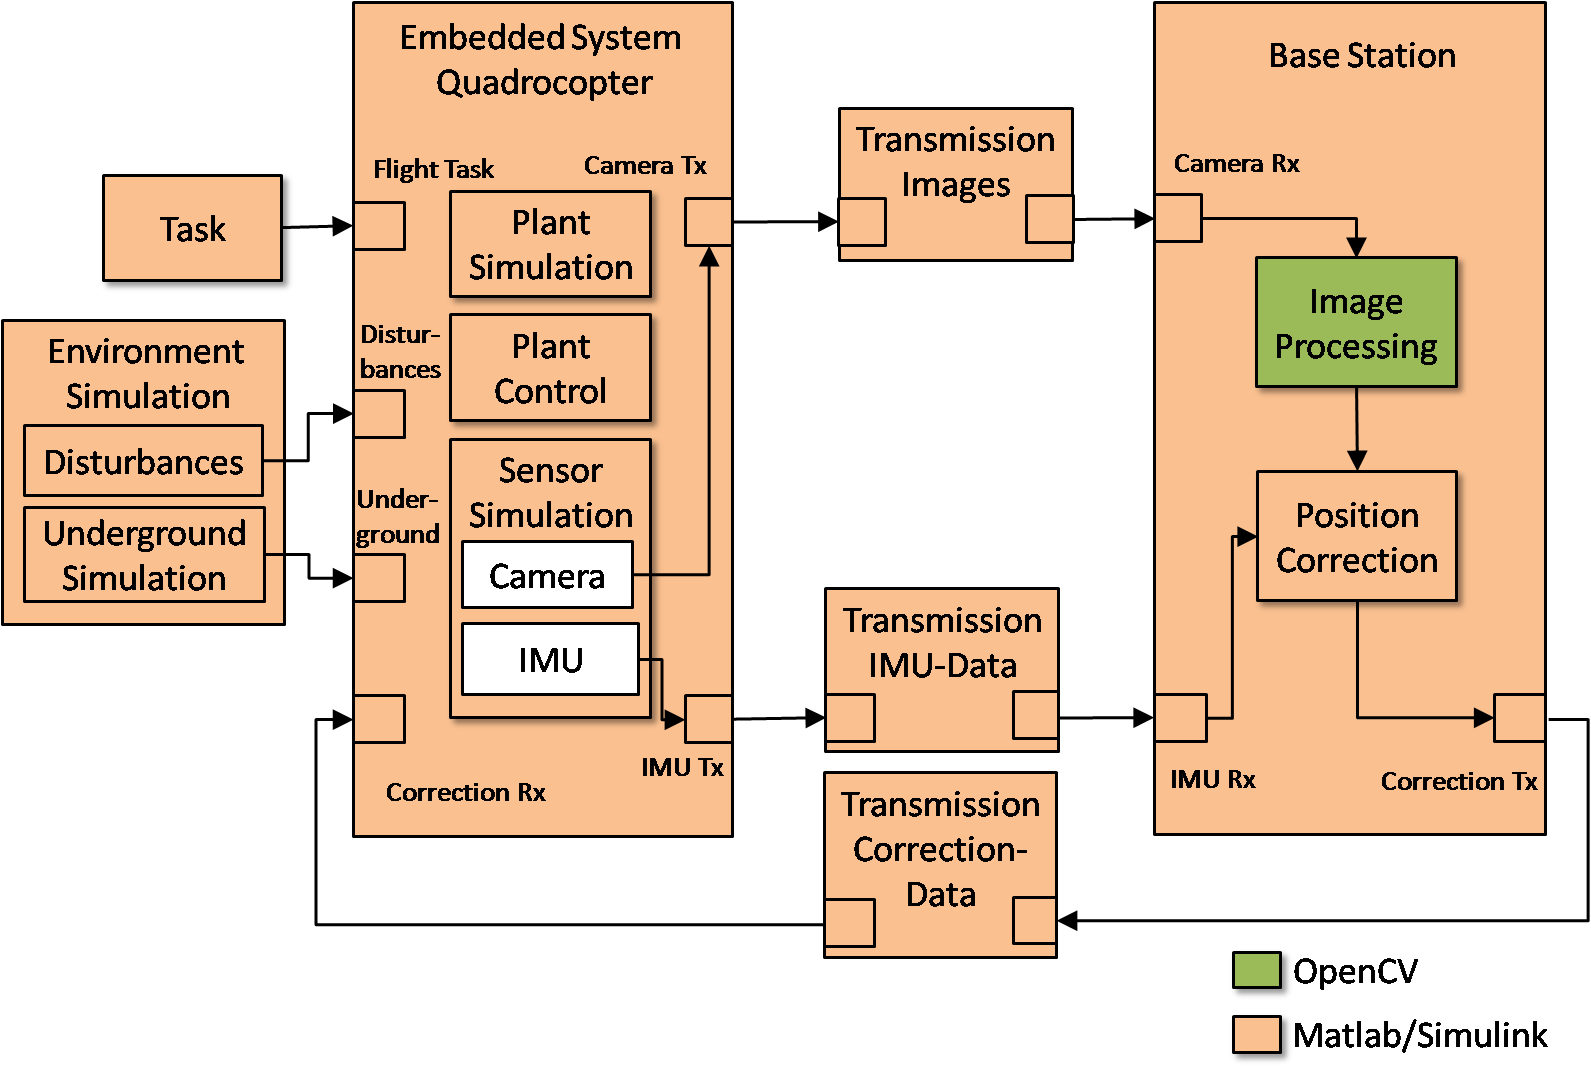
\includegraphics[width=0.75\textwidth]{graphic/InitialDesign.png}
\caption
{The Overall Design Model of the Simulation}
	\label{fig:InitialDesign}
\end{figure}

